% ---------------------------------------------------------------------
% 2.8 Inteligencia artificial y aprendizaje automático
% ---------------------------------------------------------------------
\section[INTELIGENCIA ARTIFICIAL Y APRENDIZAJE AUTOMÁTICO]{Inteligencia Artificial y aprendizaje
automático}

La inteligencia artificial (IA) es la rama de las ciencias de la computación que estudia el
diseño de agentes capaces de percibir su entorno y actuar de manera que maximicen la probabilidad
de alcanzar sus objetivos, automatizando actividades que se asocian con el pensamiento humano, como
la resolución de problemas y el aprendizaje \cite{russell2010}. No existe un método universal para
todas las áreas de aplicación de la IA, y dentro de la gran variedad de enfoques disponibles el
aprendizaje automático se ha convertido en una de sus ramas más importantes \cite{ertel2017}. A su
vez, el aprendizaje profundo es un subconjunto del aprendizaje automático basado en redes
neuronales con múltiples capas de procesamiento, relación que se ilustra en la
Figura~\ref{fig:ia}.

\begin{figure}[htbp]
\centering
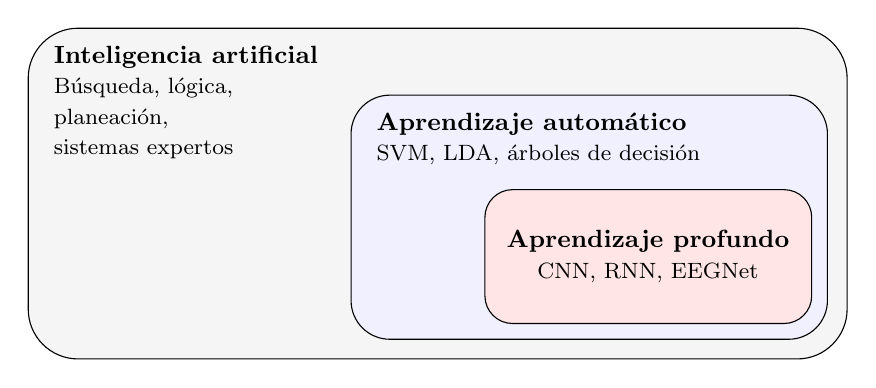
\begin{tikzpicture}[font=\small]
  \draw[fill=gray!8, rounded corners=18pt] (-5.2,-2.1) rectangle (5.2,2.1);
  \node[anchor=north west, align=left] at (-5.0,2.0) {\textbf{Inteligencia artificial}\\ \footnotesize Búsqueda, lógica,\\ \footnotesize planeación,\\ \footnotesize sistemas expertos};
  \draw[fill=blue!6, rounded corners=14pt] (-1.1,-1.85) rectangle (4.95,1.25);
  \node[anchor=north west, align=left] at (-0.9,1.15) {\textbf{Aprendizaje automático}\\ \footnotesize SVM, LDA, árboles de decisión};
  \draw[fill=red!10, rounded corners=10pt] (0.6,-1.65) rectangle (4.75,0.05);
  \node[align=center] at (2.67,-0.8) {\textbf{Aprendizaje profundo}\\ \footnotesize CNN, RNN, EEGNet};
\end{tikzpicture}
\caption{Relación entre la inteligencia artificial, el aprendizaje automático y el aprendizaje
profundo. Elaboración propia con base en \cite{goodfellow2016}.}
\label{fig:ia}
\end{figure}

\subsection{Aprendizaje automático}

En 1959, Arthur Samuel describió el aprendizaje automático como el campo de estudio que da a las
computadoras la capacidad de aprender sin ser programadas de forma explícita, a partir de su
experiencia con un programa que aprendía a jugar damas mejor que su propio creador
\cite{samuel1959}. En términos más formales, se trata de un conjunto de métodos que construyen
modelos a partir de los datos mediante el descubrimiento de patrones estadísticamente
significativos, para después aplicarlos a datos nuevos de la misma naturaleza \cite{bishop2006}.
Dependiendo de la información disponible durante el entrenamiento, se distinguen los tres tipos de
aprendizaje que se presentan en la Tabla~\ref{tab:tipos-ml}; la detección de la P300 corresponde a
un problema de clasificación binaria supervisada, pues cada época está etiquetada como objetivo o
no objetivo.

\begin{table}[htbp]
\centering
\caption{Tipos de aprendizaje automático}
\label{tab:tipos-ml}
\small
\begin{tabularx}{\textwidth}{L{2.6cm}YY}
\toprule
\textbf{Tipo} & \textbf{Descripción} & \textbf{Ejemplos de tareas} \\
\midrule
Supervisado & El modelo aprende una función que relaciona entradas con etiquetas conocidas, ajustando sus parámetros según el error entre la salida y la etiqueta. & Clasificación de épocas P300 / no P300; regresión. \\
No supervisado & El modelo busca estructura en datos sin etiquetas, agrupándolos o reduciendo su dimensión. & Agrupamiento, ICA, análisis de componentes principales. \\
Por refuerzo & Un agente aprende por prueba y error a partir de recompensas asociadas a sus acciones. & Control, juegos, adaptación en línea de una BCI. \\
\bottomrule
\end{tabularx}
\par\smallskip{\footnotesize Elaboración propia con información de \cite{bishop2006,russell2010}.}
\end{table}

\subsection{Clasificadores clásicos para la detección de la P300}

Antes del auge del aprendizaje profundo, la detección de la P300 se realizaba extrayendo
características de manera manual, generalmente las amplitudes de la señal submuestreada en cada
canal, y clasificándolas con modelos lineales. Krusienski et al. compararon cinco técnicas de
clasificación para el P300 Speller y encontraron que el análisis discriminante lineal por pasos
(SWLDA) y el discriminante lineal de Fisher ofrecían el mejor desempeño global
\cite{krusienski2006}, mientras que Rakotomamonjy y Guigue ganaron la competencia BCI III con un
conjunto de máquinas de soporte vectorial (SVM) lineales entrenadas sobre distintas particiones de
los datos \cite{rakotomamonjy2008}. En el ámbito de la ESCOM, Santos, Romero y Fernández utilizaron
el discriminante lineal de Fisher con promediado sincronizado para controlar un brazo robótico
virtual, alcanzando una precisión de 90.01\% con 20 sujetos \cite{santos2017}. La
Tabla~\ref{tab:clasicos} resume estos métodos.

\begin{table}[htbp]
\centering
\caption{Clasificadores clásicos utilizados en la detección de la P300}
\label{tab:clasicos}
\small
\begin{tabularx}{\textwidth}{L{2.4cm}YYY}
\toprule
\textbf{Clasificador} & \textbf{Descripción} & \textbf{Ventajas} & \textbf{Desventajas} \\
\midrule
LDA / Fisher \cite{krusienski2006,santos2017} & Proyecta los datos sobre la dirección que maximiza la separación entre las medias de las clases respecto a su dispersión. & Simple, rápido y con pocos parámetros; buen desempeño en P300. & Supone clases gaussianas con igual covarianza; sensible con muchas características. \\
SWLDA \cite{krusienski2006} & LDA con selección de características por pasos (se agregan o eliminan según su significancia estadística). & Reduce la dimensión y el sobreajuste; de los mejores en la comparación de \cite{krusienski2006}. & Selección costosa con muchos canales. \\
SVM lineal \cite{rakotomamonjy2008} & Busca el hiperplano que maximiza el margen entre clases. & Robusta en alta dimensión; ganó la competencia BCI III. & Requiere ajustar el parámetro de regularización; entrenamiento más lento. \\
\bottomrule
\end{tabularx}
\par\smallskip{\footnotesize Elaboración propia.}
\end{table}

\subsection{Sobreajuste y generalización}

El objetivo de un modelo de aprendizaje automático no es reproducir los datos con los que fue
entrenado sino desempeñarse correctamente con datos que nunca ha visto, capacidad conocida como
generalización \cite{goodfellow2016}. Cuando un modelo es demasiado complejo para la cantidad de
datos disponibles, o cuando se entrena durante demasiadas iteraciones, comienza a memorizar el
ruido particular del conjunto de entrenamiento: el error de entrenamiento sigue disminuyendo
mientras que el error de validación deja de bajar y empieza a crecer, fenómeno conocido como
sobreajuste y que se ilustra en la Figura~\ref{fig:sobreajuste} \cite{goodfellow2016,bishop2006}.
En el caso del EEG este riesgo es particularmente alto, pues las bases de datos suelen contener
pocos sujetos y un número limitado de épocas objetivo.

\begin{figure}[htbp]
\centering

\includegraphics[width=0.68\textwidth]{02-marco-referencial/sobreajuste.pdf}
\caption{Curvas de pérdida de entrenamiento y validación: a partir de cierto punto el modelo
comienza a sobreajustarse. Elaboración propia.}
\label{fig:sobreajuste}
\end{figure}

\subsection{Esquemas de validación}

Para estimar la capacidad de generalización, los datos se dividen en un conjunto de
entrenamiento, uno de validación, que se usa para ajustar hiperparámetros y decidir cuándo
detener el entrenamiento, y uno de prueba, que solo se utiliza al final \cite{goodfellow2016}. La
validación cruzada de $k$ particiones repite este proceso $k$ veces rotando el subconjunto de
validación, lo que ofrece una estimación más estable cuando hay pocos datos \cite{bishop2006}. En
las BCI, además, es importante distinguir entre la evaluación intrasujeto, en la que el modelo se
entrena y se prueba con datos de la misma persona, y la evaluación intersujeto, en la que se prueba
con una persona que no participó en el entrenamiento, ya sea mediante el esquema de dejar un sujeto
fuera o entrenando con sujetos distintos \cite{alvarado2021}. Contreras evaluó ambos escenarios y
obtuvo valores promedio de AUC cercanos a 0.82 en la evaluación intrasujeto y de 0.70 en la
intersujeto al considerar filas y columnas en conjunto \cite{contreras2021}.
